\documentclass{article}
\usepackage[utf8]{inputenc}
\usepackage{natbib}
\usepackage{url}
\usepackage{graphicx}
\usepackage{caption}
\usepackage[a4paper, margin=1.0cm]{geometry}

\title{
    Synthetic Data for a Model Based Learning System
\\
\begin{small}
    Joint Honours Project Plan
\end{small} 
}

\author{Sonke Wohler \\
\begin{small}
    s.wohler.15@aberdeen.ac.uk
\end{small}
}
\date{\begin{small}
    Department of Computing Science/ Department of Physics
    \\
    University of Aberdeen
\end{small}}

\pagestyle{empty}

%\bibliographystyle{unsrt}
%\bibliographystyle{abbrv}
\bibliographystyle{plain}
%\bibliographystyle{apalike}

%********************************************************************************

\begin{document}

\maketitle
\thispagestyle{empty}

\section{Context of the Project}


As with many Industries Oil and Gas is beginning to understand the value of Data and Data Analysis. \textsuperscript{\cite{chickenEgg,cloudOil}}
One possible product of such Analysis is a suitable Mathematical Model that would describe the Real World Phenomena and allow predictions about these.
Even where no additional knowledge can be gained from a Model it can improve the automation prospects for certain analysis tasks while guaranteeing transparency to the Engineers already working in the business and on the relevant projects. This sets Mathematical Models apart from other automation techniques where the inner workings of the automation are often rather opaque especially to non-Programmers. 

  \subsection{Synthetic Data}
  
Once a Model is defined it can be used to produce Synthetic Data by creating an Emulator. This Data can be used as a prediction to compare to Real Data of the Phenomenon that is to be studied. The accuracy of the prediction allows deductions about the accuracy of the Model, which in turn can be adapted and improved based on these.
\\ This process is a variation of Mathematical Modelling which forms the basis of much scientific research, in particular in the field of Physics, which it is closely associated with, but has become more common in almost any research field in recent decades, and perhaps even more so in business research.   \textsuperscript{\cite{modelling}}


  
  \subsection{Model Based Machine Learning}
  
Given the clearly defined nature of the above described Process, its automation would present an interesting prospect, as would research into the potential downsides and limitations to this Technology.
\\ Figure \ref{fig:modelLearning} describes a possible set up that could facilitate such automation, which may well be called Model Based (Machine) Learning. It can be based around an Emulator Module, which is currently for the most part programmed on demand by somebody with scientific programming expertise around a defined Model. An automated Emulator would need to produce Synthetic Data on any defined Model without having to be reprogrammed by a human.

    \begin{figure}[h]
      \centering
      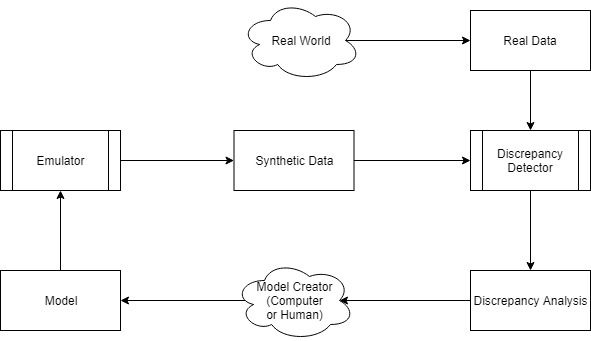
\includegraphics[width=0.7\linewidth]{figures/ModelLearning}
      \caption{A Schematic of Model Based Machine Learning}The Synthetic Data produced by the Emulator is compared against Real Data and the resulting Discreptancy Analysis informs the Model Creator in the adaptation of the Mathematical Model. Note that creating and adapting the Model is currently a Human Task, but even automation in all but this aspect may present an improvement in effectiveness of the Process.
      \label{fig:modelLearning}
  \end{figure}

\section{The Project}

The conceptual challenge to this project shall be the Concept of Model Based Machine Learning and what can be learned about its principles and limitations.
\\ Within this Concept the Emulator Module is likely the best starting point, given the relative familiarity of scientific programming. The novelty to an emulator in such a Machine Learning set up is that it cannot be build around one particular Model for a specific phenomenon. Instead it must produce an accurate Dataset based on whatever Model it is provided with, and must provide functionality for defining such a Model. This is unlike existing Emulators that are largely optimised and constrained to their particular application, and that do not allow meaningful adaptations to the Model without programmatic alterations.

  \subsection{Requirement Specifications}
  
The Student is aiming to fulfil the following Software Development Goals:

    \begin{enumerate}
      \item (Must Have) An Emulator Module that produces a set of synthetic data based on a defined, mathematical Model.
      \item (Must Have) The Emulator will offer some means for a user to define and change said Model Mathematically.
      \item (Should Have) The Emulator may provide some means for a user to define the nature of the dataset that is produced.
      \item (Should Have) The Mathematical Model definition when carried out by the user should be as user friendly as possible without compromising the Emulator's capabilities, and not require Programming experience or access.
      \item (Should Have) Sufficient and quality documentation of said Emulator to allow further development and refactoring as well as quality-assessment.
      \item (Could Have) Investigation into the capabilities and limitations of Model Based Machine Learning
      \item (Won't Have) Investigation to aid the Design of further Prototypes complementing the above Module in automating the Mathematical Modelling Processes.
      \item (Won't Have) The Emulator may provide support to the user in homogenising and comparing the synthetic data to some set of real data provided by the user.
    \end{enumerate}

  \subsection{Risk Factors and Other Considerations}

The first risk to be addressed is the potential lack of testing opportunities. While the aim of this project is only to produce a prototype, the company HyperDAP has offered some collaboration opportunities that could greatly aid the development.
\\ Concrete Data would likely be preferable as this would maximise testing capabilities, but it is equally possible that the Data this company would provide is too complex for a prototype and much simpler Models should be attempted first, with perhaps much easier possibilities for Data Acquisition.
\\ Considering its subject it is entirely possible for the project concept to fall short of expectations or prove too difficult in the long run to further pursue. However, as the aim of this project is to explore Model Based Machine Learning, the insights that may be gained will likely justify the efforts, even if no further work can be.

  \subsection{Project Timeline}
  
  Figure \ref{fig:gantt} outlines the currently intended tasks and most likely timeline with some flexibility in case of unexpected difficulties.

    \begin{figure}[h]
      \centering
      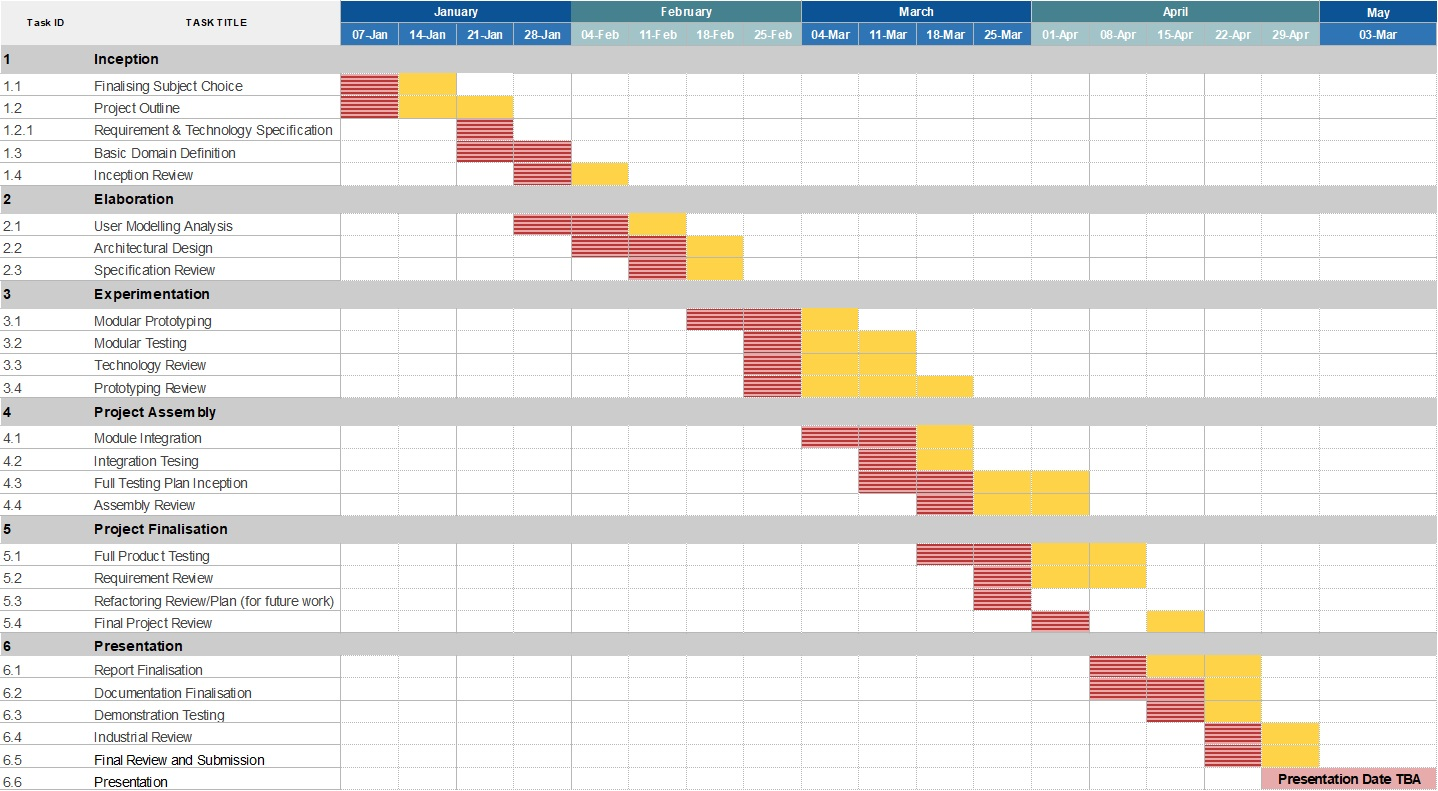
\includegraphics[width=\linewidth]{figures/ProjectPlan.jpg}
      \caption{Gantt Chart of a time-line that aims to deliver on the above specified goals.} Best case Timeline displayed in dark pink with horizontal bars, while a worst case timeline is displayed in orange. Within the confines of these timelines the project can be considered to be going according to plan. The submission date is thus far set to 03 May 2019 with a Presentation Date to be announced. Note that ideally Prototyping work should be completed by the beginning of April, and certainly leave enough time to complete project documentation and wrap-up.
      \label{fig:gantt}
    \end{figure}

\newpage

\bibliography{refs}

\end{document}
